
\label{subsec:ANN:TDNN}

As we indicated in \subsecref{neuralnetworkmodel}, prediction tasks
require the use of a dynamic neural network because of its memory
capacity. The simplest network for nonlinear prediction is the
time-delay neural network (TDNN).

TDNNs are similar to feedforward networks
(see \figref{neuralnetworkmodelVectorial}), except that the input
weight has a tap delay line (TDL) associated with
it \cite{dimith3neural}. This allows the network to have a finite
dynamic response to time series input data.

\figref{tdnn} shows an example of a TDNN, in which the dynamics appears only at the
input layer of a static multilayer feedforward network. Notice that,
in dynamic networks, the inputs and outputs of each functional block
are time dependent ($\mathbf{p}(t)$,$\mathbf{n}(t)$, $\mathbf{a}(t)$).

\begin{figure}[!ht]
\centering
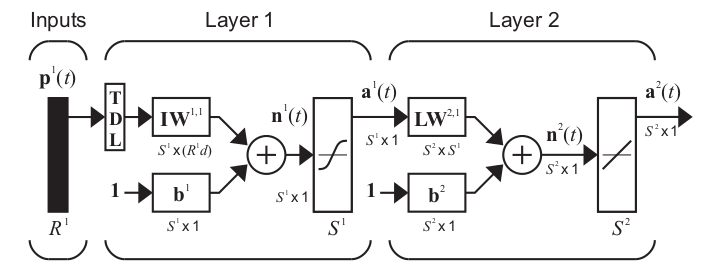
\includegraphics[width=\textwidth]{images/tdnn.png}
\caption{Time Delay network}
\label{fig:tdnn}
\end{figure}

This network has the advantage that it can be trained using exactly
the same static backpropagation algorithms
(read \secref{generalbackprop}), since the tapped-delay-line at the
input of the network can be replaced with an extended vector of
delayed values of the input.

A variant of TDNN are the distributed delay neural network, which has
delays on the layer weights in addition to the input weights.
